\chapter{Desarrollo e Implementación del Sistema Interactivo}

\section{Funcionamiento Base}

El sistema interactivo tomará en cuenta los requerimientos previos como la base de la elaboración del proyecto, si fuera necesario modificar, eliminar o añadir tareas según la exigencia de la metodología SCRUM, será en el transcurso del desarrollo.

Si bien el orden de las tareas y el procesamiento lógico puede resultar caótico, busca realizar las tareas más sencillas con el fin de profundizar el aprendizaje y enfocarse en procesos más complejos.

Para todas las pruebas iniciales realizadas se emplea el vídeo \href{https://www.youtube.com/watch?v=ymV-R5vAuQI}{I'm Han Solo Remastered}, creación de Cinematic Captures, para un sistema interactivo alternativo, seleccionado arbitrariamente por el SCRUM Team para la creación de mapas, todos los derechos a su correspondiente autor \cite{cinematiccaptures}.

\subsection{Configuración del Entorno}

\subsubsection{Características de los Equipos Personales Empleados}

La elaboración de este proyecto es realizada en 3 dispositivos distintos, dos laptops y una computadora de escritorio enfocadas para un alto rendimiento, cuyas tarjetas gráficas son de la marca nVidia Corporation, contando la GeForce GTX 960M, y dos con GeForce RTX 2060. La importancia de estos dispositivos es su capacidad de procesamiento gráfico o GPU, especializada para el desarrollo de sistemas 3D interactivos y gráficas de alta calidad, pueden llegar a ser varias veces más eficientes que la unidad central de procesamiento o CPU, en el caso de OpenPose, ejecutarlo con el CPU requiere de 8 GB de RAM, en cambio, las tarjetas gráficas tienen incorporadas memoria dedicada para el procesamiento gráfico, en el caso de OpenPose, ejecutarlo con el GPU requiere de 2 GB de memoria dedicada mínimo, siendo la cantidad disponible por la GeForce GTX 960M, cumpliendo el requisito mínimo, en cuanto a las GeForce RTX 2060, tienen una cómoda cantidad de 4 GB de memoria dedicada.

Para las cámaras de los dispositivos se emplean en el caso de las laptops, las cámaras de fábrica, que emplea la configuración genérica USB2.0 HD UVC WebCam y HD Webcam, en cuanto a la cámara de la computadora de escritorio, se emplea una cámara web genérica de orígenes desconocidos según el estudiante que la adquirió. 

El Body Tracking está implementado por la Demo.unity de manera estándar, para poder ejecutarlo en todos los dispositivos de trabajo, se debe modificar el valor de una variable que cambie la resolución del OpenPose de net\_resolution -1x176, caso contrario saltara el error más común de OpenPose \ref{erroroutofmemory} en el \ztitleref{anexoerrores}.


\subsubsection{Configuración Inicial de las SDK y herramientas}

El desarrollo de la aplicación emplea Unity y Visual Studio, ya que Visual Studio es una SDK que permite programar en C Sharp, que tiene una biblioteca disponible para el desarrollo en Unity. Además se empleará la herramienta selecta, que es el plug-in de OpenPose para poder desarrollar, el proceso de instalación se explicará en la sección de anexos. Las versiones instaladas son Unity 2019.4.14f1, Visual Studio 2019 y OpenPose 1.5.0 (la versión del plug-in de Unity, por tanto no existen más opciones disponibles actualmente).
\\
Las configuraciones son necesarias para disponer de los archivos dentro de la carpeta openpose\_plugin\textbackslash OpenPosePlugin\textbackslash Assets, en su interior se encuentran las carpetas StreamingAssets y OpenPose, dentro de la carpeta StreamingAssets se encuentran los modelos BODY\_25 y COCO, que serán necesarios para la estimación de poses. Dentro la carpeta OpenPose están las carpetas de Plugins, que contiene todas los DLL necesarios para ejecutar OpenPose, de Scripts, contiene archivos para traducir los modelos e importar los DLL respectivos y la más importante Examples, que contiene Scenes y Scripts, siendo los más relevantes. Dentro de Scripts se encuentra el código fuente del plug-in, que es modificable por el usuario y en Scenes se encuentra el Demo.unity, que provee el formato de la figura \ref{unitydemo} en \ztitleref{anexoinstalacion}.

Una vez inicializada la Demo.unity, se abre también el proyecto en C Sharp, abierto por defecto en Visual Studio 2019. Con ello, se tienen las herramientas para desarrollar el proyecto.

Siendo el primer paso la creación de un nuevo archivo.unity para el proyecto, copiando los objetos básicos del Demo.unity y relacionando la configuración de los Scripts para tener la base, se puede empezar su modificación.


\subsection{Creación del Menú}

El menú tiene 3 funciones principales:

\begin{itemize}
	\item Jugar: Un botón Play para poder entrar a la pantalla de lista de mapas.
	\item Opciones: Un botón Options para cambiar el menú principal al menú opciones cuando se lo aprieta.
	\item Salir: Un botón Quit para terminar correctamente el funcionamiento del sistema interactivo.
\end{itemize}

\subsubsection{Menú de Opciones}

El menú de opciones tiene dos funciones:
\begin{itemize}
	\item Una opción para modificar el volumen, deslizar la barra para alterar el nivel del volumen en una escala del 0 al 1 o para el usuario de 0 a 100 \%.
	\item Una opción para modificar las resoluciones, Unity permite un número de resoluciones que están registradas en su documentación, se mostraran las disponibles con el método Screen.resolutions;, su función es cambiar el largo y ancho del sistema interactivo.
\end{itemize}

\subsection{Creación de un Mapa}

La idea original sobre la creación de mapas es que el proceso de creación sea externo al sistema interactivo, de tal forma que solo tenga que añadir una carpeta con el contenido del mapa, fácilmente comprensible para el usuario que los creo y disponible para compartir entre los demás.

El método para la creación inicial de los mapas consta en 6 pasos necesarios y uno que es posiblemente útil, sin embargo, se determinará si hacerlo a futuro. Se desarrollarán dos métodos diferentes desde el paso 5, tal y como se observa en la figura \ref{pasosaseguir}. Dependiendo las dificultades y los resultados se determinará cual método conservar.

\begin{figure}[t!]
	\centering
	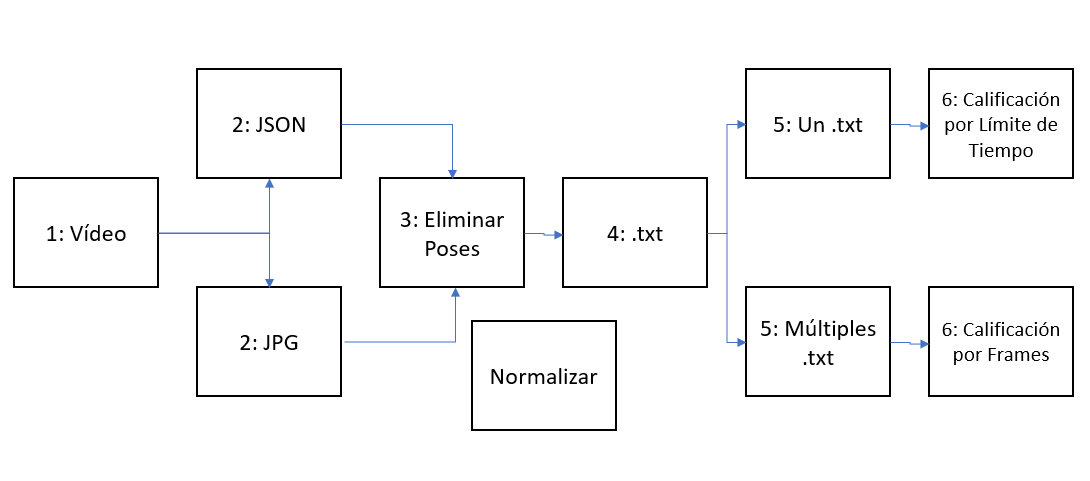
\includegraphics[width=16cm,height=7cm,]{./Images/pasosaseguir.png}
	\caption{Pasos a Seguir Para la Creación de Mapas}
	\footnotesize Fuente: Elaboración Propia
	\label{pasosaseguir}
\end{figure}

\subsubsection{Conversión de Vídeo a JSON y JPG}

El primer paso es la conversión de un vídeo grabado para la creación de un mapa y emplear un Script para ejecutar la OpenPoseDemo con la opción --write\_json output/, --number\_people\_max 1, --write\_images output\_images, --disable\_blending, --frame\_step 30 (por comodidad) y --video ./examples\_media\_hansolo.mp4, el resultado son dos carpetas llenas de archivos JSON y JPG como se ve en la figura \ref{videotojsonpjg} en el \ztitleref{anexogenerados}. 

Las opciones empleadas por la herramienta OpenPoseDemo tienen las siguientes funciones:

\begin{itemize}
	\item --write\_json dirección: Guarda los 25 puntos clave del esqueleto en un archivo JSON, se debe definir la dirección de la carpeta donde se guardarán.
	\item --write\_images dirección: Guarda los 25 puntos clave del esqueleto en un archivo JPG, se debe definir la dirección de la carpeta donde se guardarán (si no existe la carpeta donde guardar, no funcionará).
	\item --number\_people\_max X: La cantidad X límite de personas que la herramienta va a reconocer, no se reconocerán más que X, pero si menos que X si no se los reconoce.
	\item --disable\_blending: El vídeo grabado se torna negro, mostrando unicamente la pose que se reconoce.
	\item --frame\_step X: Cada cuantos Frames se guarda un JSON y JPG de una pose.
	\item --video dirección: Dirección del vídeo que se va a convertir.
\end{itemize}

\subsubsection{Eliminación de Poses}

La eliminación de poses consiste en literalmente observar los archivos JSON y JPG de cada Frame guardado, ya que comparte el número del Frame elegido al final de su nombre, se observa la imagen JPG del Frame, si no es electo para el mapa, es eliminado el JSON y JPG. Este es un proceso lento y manual ejecutado por el creador de mapas, ya que el definirá la exactitud del mapa y de las poses que desea imitar en el nivel.

\subsubsection{Conversión de JSON a txt y Almacenamiento}

Independientemente si es previa o posterior a la eliminación de poses (de preferencia posterior, ya que existen menos archivos, por tanto, es más rápido), se ejecuta un Script diseñado para convertir los archivos JSON a un formato más reconocible por el usuario. 
\\
Una vez realizada la conversión, el SCRUM Team vio dos alternativas para los archivos txt, los cuales almacenan una pose cada uno. Conservarlo como esta, siendo la carpeta donde se guardan los txt el recurso principal para recurrir a las poses del nivel o convertir todos los txt en uno solo, almacenando todas las poses en un solo txt empleando un Script, si bien almacenarlos en un solo Script es más fácil, puede que los creadores de mapas encuentren molesto la ejecución de un Script más.

\subsubsection{Adición del Tiempo Límite para Realizar las Poses}



\subsection{Comparación entre dos Poses}

Esta es considerada la tarea más compleja y laboriosa de elaborar, ya que requiere del estudio previo del modelo BODY\_25 selecto, manejo de los Scripts en C Sharp, estudio relacionado a Point Set Registration y Point Cloud. 


\subsubsection{Visualizar Movimientos del Usuario y Poses a Imitar}

La idea original consta de tres partes, observar desde el Output de la cámara al usuario y sus movimientos y mostrar al costado un vídeo cualquiera para copiar los movimientos, al estar apagada la cámara se verá en azul, como se nota en la figura \ref{primerintento}.  Se realizan modificaciones de GUI para lograrlo, este no será el producto final, es más dirigido a la facilidad de pruebas, para observar los movimientos del usuario del lado izquierdo y el vídeo a imitar del lado derecho.

\begin{figure}[t!]
	\centering
	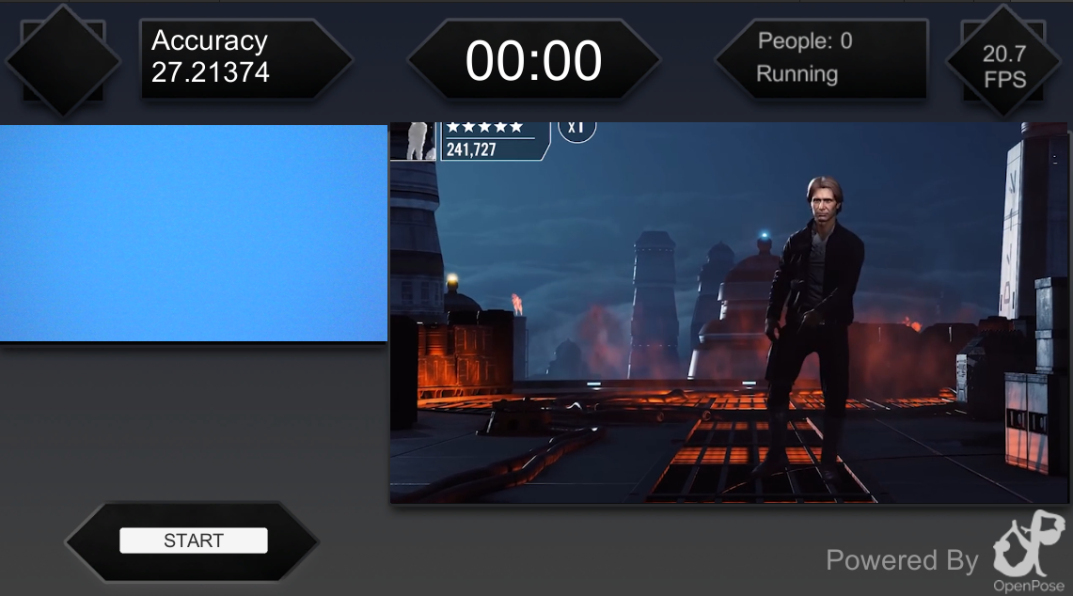
\includegraphics[width=12cm,height=7cm,]{./Images/primerintento.png}
	\caption{Primer GUI para el Desarrollo, Cambiada para el Diseño de GUI Final}
	\footnotesize Fuente: Elaboración Propia
	\label{primerintento}
\end{figure}

Adicionalmente a la visión del usuario y la pose a imitar, se debe visualizar la precisión que se tiene entre el usuario y la pose que se debe imitar, durante el desarrollo se lo empleará para revisar con los resultados de la normalización de los puntos clave la exactitud en tiempo real, calculo realizado en Normalización de Puntos Clave. 

Posteriormente, durante la inclusión del tiempo límite, se visualizará solo una comparación, siendo o la precisión adecuada para una buena calificación o la última calificación antes de pasar a la siguiente pose.

Finalmente, una vez decidido el método de normalización y la valoración de la precisión, se mostrará al usuario unicamente si sus movimientos son perfectos, buenos, malos o erróneos.

\subsubsection{Control de Tiempo del Mapa}

Se determina a través del límite de tiempo para realizar la posición que se asignó al crear el mapa, la serie de poses a imitar están en un orden específico del primero al final, por tanto el tiempo límite de cada pose es más sencillo de determinar. Durante el tiempo total del vídeo del mapa, el usuario va a poder ver una pequeña visualización de las imágenes JPG de las poses mientras ve el vídeo para poder llevar el ritmo de las poses a imitar.

Se califica la posición en el tiempo respectivo y se debe proceder a la siguiente pose cuando termine y así se mueva al nuevo tiempo límite de la siguiente pose.


\section{Normalización de Puntos Clave}

Se requiere de desarrollar un método para comparar las poses del usuario en tiempo real con las poses del mapa, para ello se obtienen en tiempo real los puntos clave del cuerpo del usuario, pero todas las personas somos distintas, por mencionar el tamaño y aparte estamos en entornos distintos, algunos pueden alinearse a la cámara, otros suelen estar o muy cerca o muy lejos, sin mencionar el espacio que tienen para moverse, pero siempre y cuando se puedan observar todos los puntos claves necesarios, se puede realizar una comparación entre poses correcta. Se debe considerar que se debe igualar lo más posible el tamaño de las poses independientemente de la posición que tengan en la pantalla y el tamaño de la persona.

El modelo BODY\_25 tiene un conjunto de puntos guardados en forma de coordenadas, lo cual se considera como un Point Cloud, por tanto, en concepto se tienen dos Point Cloud muy distintas, pero similares (ya que ambos representan un cuerpo humano) que se deben comparar, para eso existe el Point Set Registration. Durante la exploración de algoritmos inicial no se encontró ningún algoritmo para facilitar el desarrollo de la aplicación, por lo que se desarrollaron distintas formas de medir la similitud entre las poses y la precisión de los movimientos que se necesitan representar.

El método presentado es el calculo de la precisión a partir de la normalización de los puntos dentro de la Point Cloud de tres formas distintas (presentadas por cada integrante del equipo), de las cuales se definirá la más adecuada. La normalización involucra ajustar la distancia entre los puntos para que tengan distancias proporcionalmente correctas a su forma original y permitan su comparación entre dos Point Clouds distintas.


\subsection{Cálculo a partir de la Normalización de un punto}

La normalización a partir de un punto busca un punto clave como base para normalizar el resto de los puntos, del modelo BODY\_25 de la figura \ref{open2} se especificó el centro del cuerpo, el punto de la cadera central.

Se mueve el punto de la cadera central al centro de la imagen y se alinean los puntos de la persona de acuerdo a la distancia movida correspondiente como se ve en la figura \ref{overpose}. Se realizara una redimensión previa de todos los puntos existentes dentro de cada txt de las poses del mapa, se emplea la resolución 1280x720 al guardar archivos txt, cada uno de ellos será normalizado, por tanto a cada punto de las coordenadas se les aplica las ecuaciones  \ref{equation1.1} \ref{equation1.2}, donde la constante $\beta = 24$ determinado por la cantidad de puntos clave, $A_x$ es el largo y $A_y$ la altura de la resolución, P es el vector de duplas que conforman las coordenadas de la Point Cloud de la pose del usuario y Q al de la pose del mapa.
\begin{figure}[t!]
	\centering
	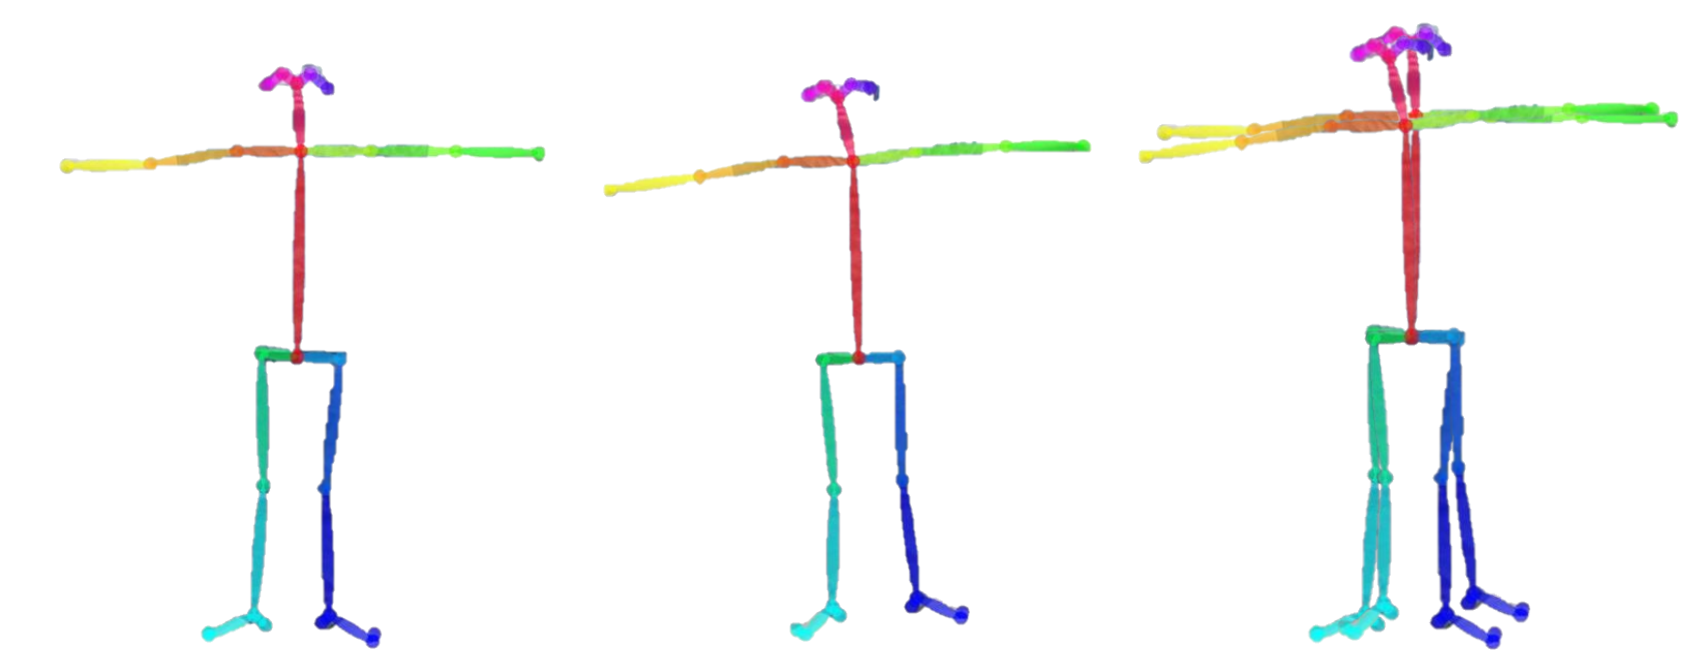
\includegraphics[width=14cm,height=6cm,]{./Images/overpose.png}
	\caption{Sobre posición de coordenadas de las poses al Centro}
	\footnotesize Fuente: Elaboración propia basado en \cite{8765346}
	\label{overpose}
\end{figure}

\begin{equation}
P=\{(\frac{x_{p0}}{A_x},\frac{y_{p0}}{A_y}),...,(\frac{x_{p\beta}}{A_x},\frac{y_{p\beta}}{A_y})\}
\label{equation1.1}
\end{equation}
\begin{equation}
Q=\{(\frac{x_{q0}}{A_x},\frac{y_{q0}}{A_y}),...,(\frac{x_{q\beta}}{A_x},\frac{y_{q\beta}}{A_y})\}
\label{equation1.2}
\end{equation}

Se calculará la distancia $N_x$ y $N_y$ \ref{equation2} que son la distancia que separa el punto de la cadera central de la otra, esos valores es la distancia que se debe recorrer en los ejes x,y para sobreponer las Point Cloud en el mismo espacio y el punto de la cadera central sobre el mismo.

\begin{equation}
N_x= x_{q8}-x_{p8} \hspace{15mm} N_y= y_{q8}-y_{p8}
\label{equation2}
\end{equation}
Se calcula el promedio del porcentaje de la diferencia de la pose del usuario a la otra con la ecuación \ref{equation3}, donde se calcula el porcentaje de diferencia de cada punto en los ejes x,y se divide el total por la cantidad de puntos clave. En la ecuación \ref{equation4} se calcula el promedio esperado de la pose del mapa.

\begin{equation}
Prom = [\sum_{n=0}^\beta (\left | (x_{pn}+N_x)*100\% \right |  +  \left |  (y_{pn}+N_y)*100\%  \right |) ]/\beta
\label{equation3}
\end{equation}

\begin{equation}
ExpProm = (\sum_{n=0}^\beta (\left | (x_{qn}+y_{qn})*100\% \right |))/\beta
\label{equation4}
\end{equation}

Finalmente se calcula el porcentaje de error que existe entre las dos poses en la ecuación \ref{equation6}. 

\begin{equation}
Acurracy = 100 - (\frac{Prom}{ExpProm})*100 \%
\label{equation6}
\end{equation}



Un ejemplo es desarrollado en el \ztitleref{anexocadera}, donde dadas 8 poses de 8 Frames de una grabación de prueba donde se realizan distintas pruebas, son comparadas y se concluye que calcular el promedio de diferencia entre dos poses no es una solución optima, pues un brazo puede estar totalmente fuera de lugar, pero al promediar todos los porcentajes de error se minimiza el efecto de la diferencia del brazo, que es muy importante. Por tanto este método de cálculo queda descartado.


\subsection{Cálculo a partir de la Normalización de Cuadro de Point Cloud}

Para la normalización del cuadro de Point Cloud, se busca los mínimos $X_min$ y los máximos $X_max$ del conjunto de puntos en las Point Clouds del usuario y de la pose guardada en el mapa \ref{equation12.max} \ref{equation12.min} \ref{equation14.max} \ref{equation14.min}.
\begin{equation}
X_{pmax} = Max(P(x_p)) \hspace{15mm} Y_{pmax} = Max(P(y_p))
\label{equation12.max}
\end{equation}
\begin{equation}
X_{pmin} = Min(P(x_p)) \hspace{15mm} Y_{pmin} = Min(P(y_p))
\label{equation12.min}
\end{equation}
\begin{equation}
X_{qmax} = Max(Q(x_q)) \hspace{15mm} Y_{qmax} = Max(Q(y_q))
\label{equation14.max}
\end{equation}
\begin{equation}
X_{qmin} = Min(Q(x_q)) \hspace{15mm} Y_{qmin} = Min(Q(y_q))
\label{equation14.min}
\end{equation}
Los mínimos y máximos se convierten en los bordes limitantes de un cuadro imaginario que los encierra, como se ve en la figura \ref{pointcloudtocuadro} otorgando un tamaño del conjunto de los puntos, con ello se puede redimensionar el Point Cloud de la pose del usuario al tamaño de la Point Cloud de la pose del mapa con que se compara como se ve en la figura \ref{redimensioncuadro}, para evaluar el desfase porcentual que existen en los ejes x,y de cada punto.

\begin{figure}[t!]
	\centering
	\begin{subfigure}{.5\textwidth}
		\centering
		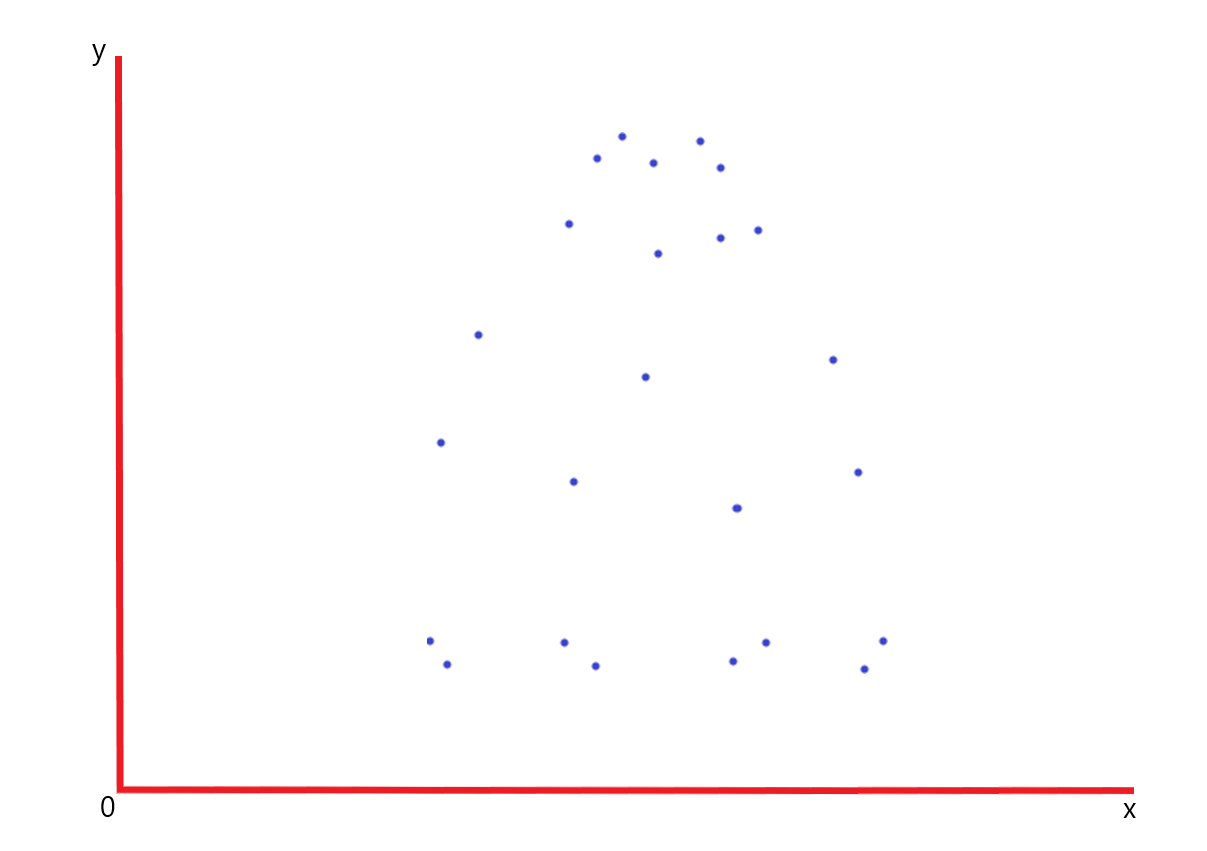
\includegraphics[width=7cm,height=5cm,]{./Images/pointcloud.png}
		\caption{Ejemplo de Point Cloud}
		\label{pointcloud}
	\end{subfigure}%
	\begin{subfigure}{.5\textwidth}
		\centering
		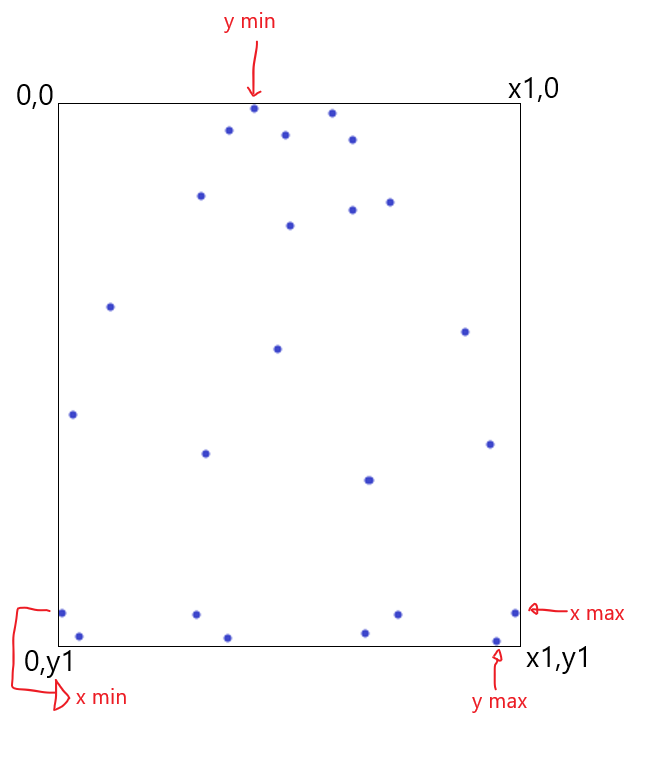
\includegraphics[width=5cm,height=5cm]{./Images/cuadropointcloud1.png}
		\caption{Cuadro de la Point Cloud}
		\label{cuadro}
	\end{subfigure}
	\caption{Ejemplos de Encuadre de una Point Cloud}
	\footnotesize Fuente: Elaboración propia
	\label{pointcloudtocuadro}
\end{figure}


\begin{figure}[t!]
	\centering
	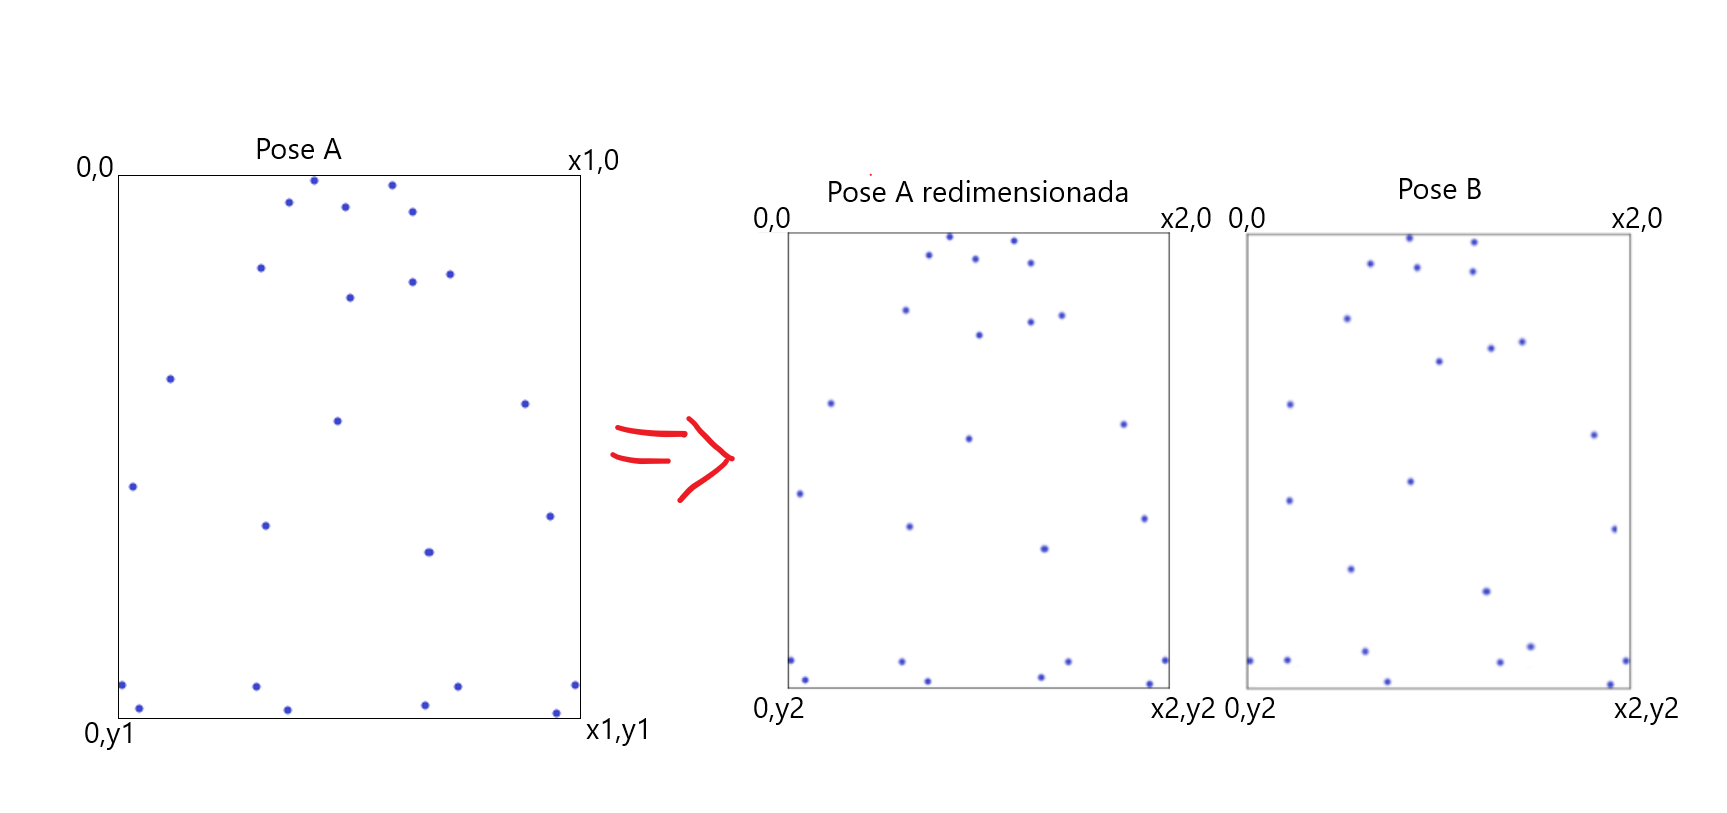
\includegraphics[width=14cm,height=6cm,]{./Images/redimensioncuadro.png}
	\caption{Redimensionamiento de la Point Cloud A al tamaño de la Point Cloud B}
	\footnotesize Fuente: Elaboración propia
	\label{redimensioncuadro}
\end{figure}

Se calcula el límite entre los dos extremos en $x_size$ y $y_size$ de cada pose \ref{equation15.1} \ref{equation15.2} y se calcula una constante de proporción $\sigma$ y $\varphi$ \ref{equation16} para los ejes x,y que permitirá comparar la distancia de cada pose respecto a la de la otra pose.

\begin{equation}
(x_{psize},y_{psize}) = ((x_{pmax}-x_{pmin}),(y_{pmax}-y_{pmin}))
\label{equation15.1}
\end{equation}
\begin{equation}
(x_{qsize},y_{qize}) = ((x_{qmax}-x_{qmin}),(y_{qmax}-y_{qmin}))
\label{equation15.2}
\end{equation}
\begin{equation}
\sigma = \frac{x_{psize}}{x_{qsize}} \hspace{15mm} \varphi = \frac{y_{psize}}{y_{qsize}}  
\label{equation16}
\end{equation}

Se calcula la precisión en la variable $Acurracy$ \ref{equation19}, la cual será la sumatoria del cálculo de la diferencia porcentual de cada punto modificada para tener un valor exponencial de acuerdo al porcentaje de diferencia. Donde la constante $\beta = 24$ debido a la cantidad de puntos clave, $C$ \ref{equation18.1} y $D$ \ref{equation18.2} son la varianza exponencial de los valores $A$ \ref{equation17.1} y $B$ \ref{equation17.2}, que son el porcentaje de diferencia entre dos poses tomando en cuenta la proporcionalidad.

\begin{equation}
Acurracy = \sum_{n=0}^\beta (\left | C \right |  +  \left |  D \right |) 
\label{equation19}
\end{equation}

\begin{equation}
A=(\frac{x_{pn}-x_{qn}*\sigma}{x_{qsize}} *100 \% )
\label{equation17.1}
\end{equation}
\begin{equation}
B=(\frac{y_{pn}-y_{qn}*\varphi}{y_{qsize}} *100 \% )
\label{equation17.2}
\end{equation}

\begin{equation}
C=\left\{\begin{matrix}
A^{\log A} , si \hspace{2mm} A \geq 1  \\
A , si \hspace{2mm} A <  1
\end{matrix}\right. 
\label{equation18.1}
\end{equation}

\begin{equation}
D=\left\{\begin{matrix}
B^{\log B} , si \hspace{2mm} B \geq 1  \\
B , si \hspace{2mm} B <  1
\end{matrix}\right.
\label{equation18.2}
\end{equation}

El rango de la precisión de cada punto sería de $0 \leq x \geq 10000$ para un total de $0 \leq x \geq 250000$ del valor de $Acurracy$, siendo el 0 la comparación entre dos poses iguales y 250000 siendo todos los puntos de una pose en un extremo y los de la otra pose en el otro extremo en ambos ejes, lo cual es imposible en el contexto. Sin embargo, la volatilidad al tener un error en un punto especifico no es lo suficientemente alta, por tanto, este método de cálculo fue descartado.

 
\subsection{Cálculo a partir de la Normalización de la distancia entre dos puntos}

La normalización a partir de la distancia cuenta con una constante $\beta = 24\text{ Key Points}$ (ya que va del 0 al 24)entre dos puntos elige dos puntos del modelo BODY\_25 de la figura \ref{open2}, el punto del cuello (Punto 1) y el punto de la cadera central (Punto 8), ya que conforman la línea principal del cuerpo que une extremidades inferiores y superiores. Se obtiene una constante a partir de la división de las distancias de ambas poses a comparar que permite acomodar la posición de los demás puntos 

Se convertirá a las Point Cloud como un vector de duplas x,y de la siguiente forma $P=\{(x_{p0},y_{p0}),...,(x_{p\beta},y_{p\beta})\}$ y $Q=\{(x_{q0},y_{q0}),...,(x_{q\beta},y_{q\beta})\}$
, donde P es el vector del usuario y Q es de la pose del mapa, $x_{pn}$ es un valor del vector, que respeta el  orden de la tabla \ref{openposevector}. Se debe calcular las distancias $d_p$ y $d_q$ que hay entre los puntos clave mencionados (cuello y cadera central) con la ecuación $d_p= distancia((x_{p1},y_{p1}),(x_{p8},y_{p8}))$ y $d_q= distancia((x_{q1},y_{q1}),(x_{q8},y_{q8}))$.

Se calcula una constante que determina la proporción entre las distancias entre el usuario respecto a la pose del mapa \ref{equation8}, esto nos permitirá definir la diferencia entre las distancias del punto del cuello de la pose del usuario respecto a la de la pose del mapa en las ecuaciones \ref{equation9.1} y \ref{equation9.2}. La distancia $D_x$ y $D_y$ determinan la lejanía del punto del cuello respecto al otro punto del cuello en el cuadro de la pose basándose en sus proporciones.
\begin{equation}
\gamma = \frac{d_p}{d_q}
\label{equation8}
\end{equation}
\begin{equation}
D_x= (x_{p1}*\gamma - x_{q1})
\label{equation9.1}
\end{equation}
\begin{equation}
D_y= (y_{p1}*\gamma - y_{q1})
\label{equation9.2}
\end{equation}

Finalmente, se calculará la diferencia que existe entre cada punto normalizado de la pose del usuario y los puntos de la pose del mapa, se resta $D_x$ y $D_y$ para sobreponer los ejes de las coordenadas de cada punto en la ecuación \ref{equation10} para obtener la diferencia entre una pose de otra. 
\begin{equation}
Acurracy = D_{sum} = \sum_{n=0}^\beta (\left | x_{pn}*\gamma -x_{qn}-D_x \right |+\left | y_{pn}*\gamma -y_{qn}-D_y \right |) 
\label{equation10}
\end{equation}

El resultado varía bastante dependiendo de la resolución de la cámara. Se estima un rango de Acurracy entre $ 500 < x \geq 1000000$, al ser tan amplio el rango, cuando se mueve un punto fuera de lugar el cambio de la precisión es elevado, por tanto, este es el método de calculo seleccionado.



\section{Diseño De GUI}

El diseño de la GUI de la figura \ref{requerimientosgrafico} en la fase de diseño se tomó en cuenta para su creación, donde se tienen los botones y funciones esperadas. Para el diseño también se toma en cuenta el principio KISS ("Keep it Simple, Stupid!"), que establece que gran parte de los sistemas son mejores si se mantienen simple que complejos, este se vuelve un objetivo clave para el diseño de la GUI.
\\
La licencia de OpenPose específica la necesidad de mantener en claro que el uso de la API esta dirigido a investigación y desarrollo privado, perteneciendo a su creador todos los programas desarrollados con su uso.
Se resalta también que a estas etapas del desarrollo recién \textbf{se determinó el nombre del sistema interactivo POSE IT!}, en la figura \ref{menu} se observan los logos de POSE IT! y de OpenPose, así mismo las 3 funciones mencionadas.

\begin{figure}[h!]
	\centering
	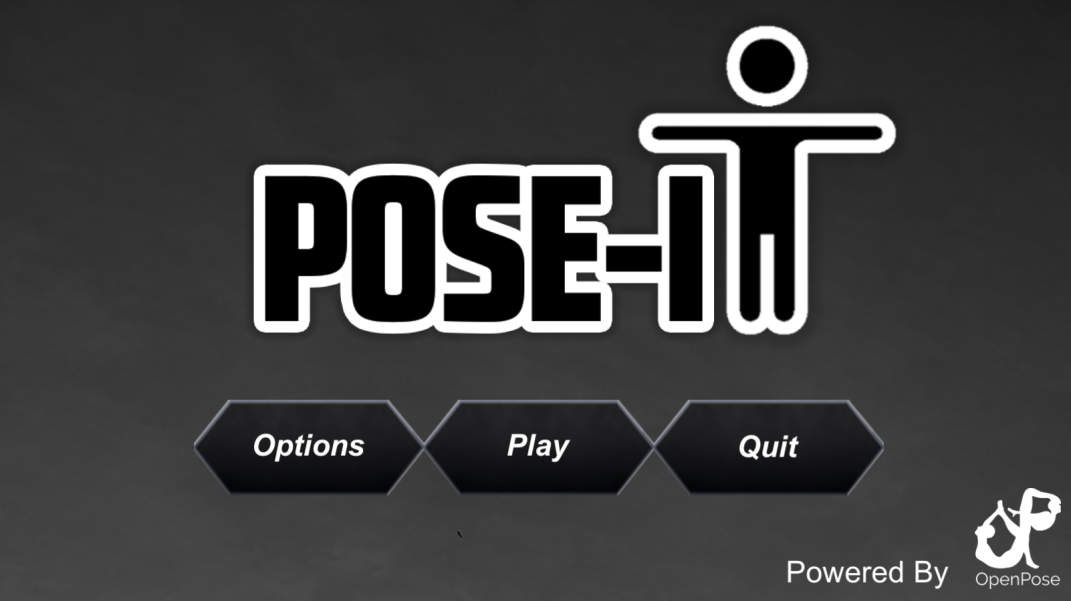
\includegraphics[width=12cm,height=7cm]{./Images/menu.png}
	\caption{Menú de el Sistema Interactivo POSE IT!}
	\footnotesize Fuente: Elaboración Propia
	\label{menu}
\end{figure}

Al presionar Options en la figura \ref{menu}se observan las dos funciones observadas funcionales marcadas en rojo de la figura \ref{menuoptions}, así mismo se añadió la posibilidad de poner la pantalla en modo "Fullscreen", que en español es pantalla completa.

\begin{figure}[t!]
	\centering
	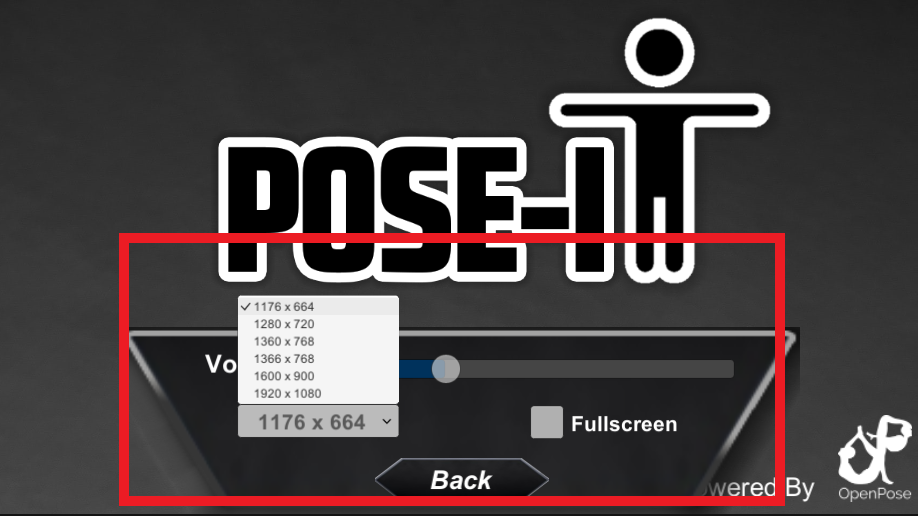
\includegraphics[width=12cm,height=7cm]{./Images/menuopciones.png}
	\caption{Menú de Opciones}
	\footnotesize Fuente: Elaboración Propia
	\label{menuoptions}
\end{figure}

Al apretar Play de la figura \ref{menu} se pueden observar la lista de mapas disponibles, existen dos botones marcados en rojo en la figura \ref{menulistas} para "Volver" al menú principal \ref{menu} o para iniciar a interactuar con el mapa elegido.Marcado en verde, se puede apreciar la lista de mapas disponibles, que al seleccionar un mapa, se escuchará levemente el audio del mapa, si es configurado, en la parte marcada con azul, se verá también el nombre del mapa, el autor que creo la pieza, el grupo que lo toco y quien creo el mapa.

\begin{figure}[t!]
	\centering
	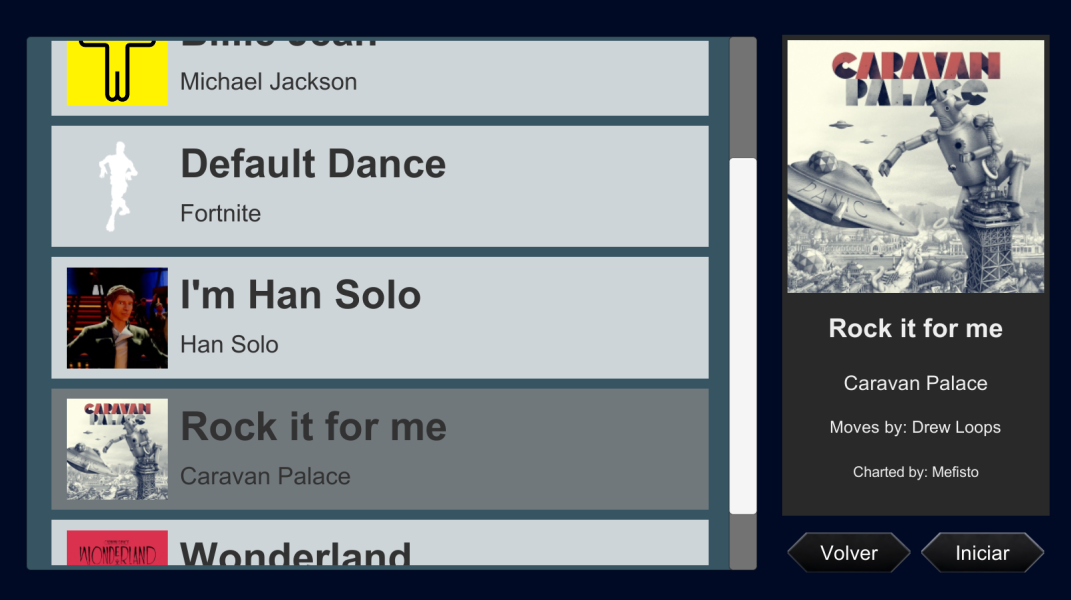
\includegraphics[width=12cm,height=7cm]{./Images/menudelistas.png}
	\caption{Menú de Listas para Mapas de POSE IT!}
	\footnotesize Fuente: Elaboración Propia
	\label{menulistas}
\end{figure}

\section{Modificación de Requerimientos Adicionales debido a SCRUM}

La metodología SCRUM









